\documentclass[11pt,a4paper]{uebung}

\usepackage[british]{babel}
\usepackage{epsfig}
\usepackage{rotate}
\usepackage{amsmath,amsthm,amssymb}
\usepackage{color}
\makeatletter\let\@amsfonts=P\makeatother
\usepackage{graphicx}
\usepackage{typearea}
\usepackage{multicol}
\usepackage{amsfonts}
\usepackage[nounderscore]{syntax}
\usepackage{enumitem}
%\usepackage{paralist}
\newcommand{\comment}[1]{\marginpar{\small{\bf Comment:} #1}}


\usepackage{tikz}
\usetikzlibrary{shapes,arrows,backgrounds,%
matrix,patterns,arrows,decorations.pathmorphing,decorations.pathreplacing,%
positioning,fit,calc,decorations.text,shadows%
}

\newcommand{\solution}[1]{\par {\bf Solution:}\\#1}



%put your Matrikelnummer here instead of the XXXXXXXX
% if your group has less than 3 members, just delete the remaining XXXXXXXX
\newcommand\matrikelnummerA[0]{0603596}
\newcommand\matrikelnummerB[0]{0727156}
\newcommand\matrikelnummerC[0]{0725146}
%put your Matrikelnummer here instead of the XXXXXXXX



\def\cT{\mathcal{T}}


\begin{document}
\newcommand{\Vorlesung}{Formal Methods in Computer Science}
\newcommand{\Semester}{SS 2012}
\newcommand{\Prof}{Uwe Egly}
\newcommand{\AssisA}{Antonius Weinzierl}
\newcommand{\AssisB}{}

%%%%%%%%%%%%%%%%%%%%%%%%%%%%%%%%%%%%%%%%%%%%%%%%%%%%%%%%%%%%%%%%%%%%%%%%%%%%%%

\Uebungsblatt{2 (10 points)}{
  \begin{tabular}{rl}
   Matrikelnummer(n): &\matrikelnummerA \\
   &\matrikelnummerB \\
   &\matrikelnummerC
  \end{tabular}
}

%%%%%%%%%%%%%%%%%%%%%%%%%%%%%%%%%%%%%%%%%%%%%%%%%%%%%%%%%%%%%%%%%%%%%%%%%%%%%%


\newcommand{\lr}{\leftrightarrow}
\newcommand{\la}{\leftarrow}
\newcommand{\ra}{\rightarrow}
\newcommand{\xor}{\oplus}
\newcommand{\li}{l_{i}}
\newcommand{\lia}{l_{i_1}}
\newcommand{\lib}{l_{i_2}}
\newcommand{\lk}{l_{k}}
\newcommand{\lka}{l_{k_1}}
\newcommand{\lkb}{l_{k_2}}

\Aufgabe[Tseitin Transformation \hfill \bf (0.5 + 1 + 1.5 points)]

\begin{enumerate}
\item Extend Tseitin's transformation for the connectives $\leftrightarrow$
  (equivalence) and $\oplus$ (XOR). Find the necessary clauses for the new schemes
  $l_i \leftrightarrow (l_{i_1} \leftrightarrow l_{i_2})$ and $l_k
  \leftrightarrow (l_{k_1} \oplus l_{k_2})$.
  
  \solution{    \begin{itemize}
    \item $\li \lr (\lia \lr \lib)$
      
      First we have to use some simple simplification we obtain clauses $(1)$ and $(2)$:
      \begin{align*}
        \li \lr& (\lia \lr \lib) \\
        \equiv \li \lr& (\lia \ra \lib \land \lib \ra \lia)\\
        \equiv \li \ra& (\lia \ra \lib \land \lib \ra \lia)\; \land\\
        & (\lia \ra \lib \land \lib \ra \lia) \ra \li
      \end{align*}
      To ensure that we don´t lose the overview about the formulas we split the formula into two subcases:
        \begin{align*}
      \tag{1} \li \ra  (\lia \ra \lib \land \lib \ra \lia) \\
      \tag{2}  (\lia \ra \lib \land \lib \ra \lia) \ra \li
        \end{align*}

    %We derive the first two clauses $C_{1}=(\neg\li\lor\neg\lia \lor
     %\lib)$ and $C_{2}=(\neg\li\lor\neg\lib \lor \lia)$ from $(*)$ as follows:
     For the first formula
      \begin{align*}
        \tag{1}&\li \ra (\lia \ra \lib \land \lib \ra \lia)\\
        \equiv & \li \ra (\neg\lia \lor \lib) \land \li\ra (\neg\lib \lor \lia) \\
        \equiv &(\neg\li\lor\neg\lia \lor \lib) \land (\neg\li\lor\neg\lib \lor \lia)
      \end{align*}
    So we can derive the first two clauses $C_{1}=(\neg\li\lor\neg\lia \lor
    \lib)$ and $C_{2}=(\neg\li\lor\neg\lib \lor \lia)$ 

     For the second formula we can calculate the following clauses:
      \begin{align*}
        \tag{2}& (\lia \ra \lib \land \lib \ra \lia) \ra \li\\
        \equiv &\neg((\neg\lia\lor\lib) \land (\neg\lib \lor \lia))
        \lor \li\\
        \tag {rule 2}\equiv &((\lia\land\neg\lib)\lor(\lib\land\neg\lia))\lor\li \\
        \tag {rule 2}\equiv &((\lia \lor(\lib \land
        \neg\lia)\land(\neg\lib\lor(\lib\lor\neg\lia)))\lor\li  \\
        \tag {rule 1}\equiv & ((\lia \lor \lib) \land (\lia \lor \neg\lia) \land
        (\neg\lib \lor \lib) \land (\neg\lib \lor \neg\lia)) \lor
        \li  \\
        \equiv & (\li \lor \lia \lor \lib) \land (\li \lor \neg\lib \lor \neg\lia)
      \end{align*}
      So we derive the next two clauses $C_{3}=(\li \lor \lia \lor \lib)$
      and $C_{4}=(\li \lor \neg\lib \lor \neg\lia)$ and the we are finished for the equivalence.
 \bigskip 
    
    \item $\lk \lr \lka \xor \lkb$
      
     Once again we use the subformulas $(1)$ and $(2)$ to abtain the clauses after the first simplifications:
      \begin{align*}
        \lk \lr& (\lka \xor \lkb) \\
        \equiv \lk \lr& (\lka \lor \lkb) \land (\neg\lka \lor \neg\lkb)\\
        \tag{1}\equiv \lk \ra& ((\lka \lor \lkb) \land (\neg\lka \lor \neg\lkb))\; \land\\
        \tag{2}& \neg((\lka \lor \lkb) \land (\neg\lka \lor \neg\lkb)) \ra \lk
      \end{align*}
      We derive the first two clauses from $(1)$ in with the following steps: (same steps as above)
     
      \begin{align*}
        \tag{1}&\lk \ra ((\lka \lor \lkb) \land (\neg\lka \lor \neg\lkb))\\
        \equiv &(\neg\lk\lor\lka\lor\lkb) \land (\neg\lk\lor\neg\lka\lor\neg\lkb)    
      \end{align*}
      $C_{1}=(\neg\lk\lor\lka\lor\lkb)$ and
      $C_{2}=(\neg\lk\lor\neg\lka\lor\neg\lkb)$ 
     
     For the second formula we can calculate the following clauses:
      follows:
      \begin{align*}
        \tag{2}& \neg((\lka \lor \lkb) \land (\neg\lka \lor
        \neg\lkb)) \ra \lk\\
        \equiv & ((\neg\lka \land \neg\lkb) \lor (\lka \land
        \lkb))\lor \lk\\
        \equiv & (((\lka \lor (\neg\lka\land\neg\lkb)) \land (\lkb
        \lor (\neg\lka\land\neg\lkb)))\lor \lk\\
        \equiv & ((\lka \lor\neg\lkb) \land (\neg\lka\lor\lkb)) \lor
        \lk\\
        \equiv & (\lk \lor \lka \lor\neg\lkb) \land (\lk \lor \neg\lka\lor\lkb)
      \end{align*}
      Finally we derive the clauses 
      $C_{3}=(\lk \lor \lka \lor\neg\lkb)$
      and $C_{4}=(\lk \lor \neg\lka\lor\lkb)$ from $(2)$ and we are finished.
    \end{itemize} 
  }

\item Apply Tseitin's transformation to the following formula $\psi$: $a \rightarrow
  \big( b \lor \neg (a \leftrightarrow c)\big)$.

  
  Hint: You do not need to introduce labels for propositions $a,b,$ and $c$.
  \solution{
For the first step we have to generate a formula tree as follows (see Fig 1 ):
We don´t need to introduce labels for the propositional formulas so we can define the following equivalences from the formula tree:
    \begin{align*}
      l_1 &\lr (a \lr c)\\
      l_2 &\lr (\neg l_{1})\\
      l_3 &\lr (b \lor l_{2})\\
      l_4 &\lr (a \ra l_{3})\\
    \end{align*}

In the next step we create a Table and to Translate the “labeling formulas” to clauses:

    \begin{table}[ht]
      \centering
      \begin{tabular}{l|cccc}
        & $C_{1}$ & $C_{2}$ & $C_{3}$ & $C_{4}$ \\
        \hline
        $l_1 \lr (a \lr c)$ & $\neg l_{1},\neg a,c$ & $\neg l_{1}, a,
        \neg c$ & $l_{1}, a, c$ & $l_{1},\neg a, \neg c$\\
        $l_{2}\lr (\neg l_{1})$& $l_{1},l_{2}$ & $\neg l_{1}, \neg
        l_{2}$ & $TRUE$ & $TRUE$\\
        $l_3 \lr (b \lor l_{2})$ & $\neg l_{3},b,l_{2}$ & $\neg b,
        l_{3}$ & $\neg l_{2},l_{3}$ &$TRUE$\\
        $l_4 \lr (a \ra l_{3})$ & $\neg l_{4}, \neg a, l_{3}$ &
        $l_{4},a$ & $l_{4}, \neg l_{3}$&$TRUE$
      \end{tabular}
      \caption{Clause set resulting from the Tseitin transformation to $\psi$}
      \label{tab:tseitin}
    \end{table}

    \begin{figure}[ht]
      \centering
      \begin{tikzpicture}
        \node[label={[green]above:$l_4$}] {$\ra$}
        child {
          node {$a$}
        }
        child {
          node[label={[green]right:$l_3$}] {$\lor$}
          child {
            node {$b$}
          }
          child {
            node[label={[green]right:$l_2$}] {$\neg$}
            child {
              node[label={[green]right:$l_1$}] {$\lr$}
              child {
                node {$a$}
              }
              child {
                node {$c$}
              }
            }
          }
        }
        ;
      \end{tikzpicture}
      \caption{Formula tree for the corresponding formula (the need labels are colored green)}
      \label{fig1}
    \end{figure}

  }


\item Let $\psi$ be a propositional formula and $D^\psi$ the set of clauses
  resulting from Tseitin's transformation on $\psi$. Prove that the following
  holds:
  
  \centerline{If $\psi$ is satisfiable then $D^\psi$ is satisfiable.}

  You only need to prove this for the connectives $\land$ and $\neg$.
  %\lor,\neg, \rightarrow$.
  Use the below clause schemes, which introduce a new label for every boolean
  variable.
  \begin{align*}
    L_a \leftrightarrow a && (\neg L_a \lor a)&& (L_a \lor \neg a)\\
    L_\phi \leftrightarrow (L_1 \land L_2) && (\neg L_\phi \lor L_1)&& (\neg
    L_\phi \lor L_2)&& (L_\phi \lor \neg L_1 \lor \neg L_2)\\
    L_\phi \leftrightarrow \neg L_1 && (\neg L_\phi \lor \neg L_1)&& (L_\phi
    \lor L_1)
  \end{align*}
  
  \solution{
  }
\end{enumerate}


%%%%%%%%%%%%%%%%%%%%%%%%%%%%%%%%%%%%%%%%%%%%%%%%%%%%%%%%%%%%%%%%%%%%%%%%%%%%%%

\newpage
\Aufgabe[Implication Graphs \hfill \bf (2+1+1.5 points)]
\begin{enumerate}
\item Let $\mathcal{D}$ be the following set of clauses:
  \begin{align*}
    c_1:& (A \lor B)\\
    c_2:& (A \lor G \lor H)\\
    c_3:& (\neg B \lor \neg D \lor E)\\
    c_4:& (E \lor F)\\
    c_5:& (\neg F \lor \neg G \lor D)\\
    c_6:& (\neg C \lor G \lor J)\\
    c_7:& (\neg J \lor \neg H)
  \end{align*}
  Draw the implication graph resulting from $\mathcal{D}$ with decisions
  $A=0@1$, $C=1@2$, $E=0@3$. Find the first UIP, and learn a new clause using
  the first-UIP scheme (use resolution).

  \solution{
  \begin{figure}[h]
    \centering
    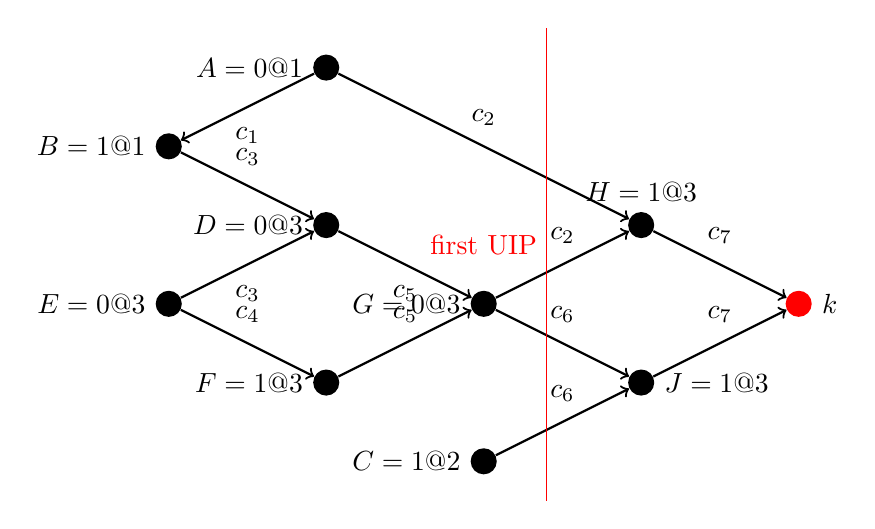
\begin{tikzpicture}
      \coordinate (A) at (0,2);
      \coordinate (B) at (-2,1);
      \coordinate (C) at (2,-3);
      \coordinate (D) at (0,0);
      \coordinate (E) at (-2,-1);
      \coordinate (F) at (0,-2);
      \coordinate (G) at (2,-1);
      \coordinate (H) at (4,0);
      \coordinate (J) at (4,-2);
      \coordinate (K) at (6,-1);
      %\coordinate (L) at (2,-1);
      
      \node[fill,circle,label=left:{$A=0@1$}] (ab) at (A) {};
      \node[fill,circle,label=left:{$B=1@1$}] (bd) at (B) {};
      \node[fill,circle,label=left:{$C=1@2$}] (cj) at (C) {};
      \node[fill,circle,label=left:{$D=0@3$}] (dg) at (D) {};
      \node[fill,circle,label=left:{$E=0@3$}] (ed) at (E) {};
      \node[fill,circle,label=left:{$F=1@3$}] (fg) at (F) {};
      \node[fill,circle,label=left:{$G=0@3$}] (gh) at (G) {};
      \node[fill,circle,label=above:{$H=1@3$}] (hk) at (H) {};
      \node[fill,circle,label=right:{$J=1@3$}] (jk) at (J) {};
      \node[fill,circle,label=right:{$k$},red] (kk) at (K) {};
      %\node[red,label=above:{$first UIP$}] (ll) at (L) {};
      \node [above, red] at (2,-0.5) {first UIP};
      
      \draw[->,thick] (ab) --node[label=below:$c_1$] {} (bd);
      \draw[->,thick] (bd) --node[label=above:$c_3$] {} (dg);
      \draw[->,thick] (ed) --node[label=below:$c_3$] {} (dg);
      \draw[->,thick] (ed) --node[label=above:$c_4$] {} (fg);
      \draw[->,thick] (dg) --node[label=below:$c_5$] {} (gh);
      \draw[->,thick] (fg) --node[label=above:$c_5$] {} (gh);
      \draw[->,thick] (gh) --node[label=above:$c_2$] {} (hk);
      \draw[->,thick] (gh) --node[label=above:$c_6$] {} (jk);
      \draw[->,thick] (cj) --node[label=above:$c_6$] {} (jk);
      \draw[->,thick] (jk) --node[label=above:$c_7$] {} (kk);
      \draw[->,thick] (hk) --node[label=above:$c_7$] {} (kk);
      \draw[->,thick] (ab) --node[label=above:$c_2$] {} (hk);
      
      \draw [red](2.8,2.5) -- (2.8,-3.5);
      

    \end{tikzpicture}
    \caption{Implication Graph}
    \label{fig:ig}
  \end{figure}
  
  We have two UIP's in this implication graph. The decision node (in this case E) is always an UIP, but the first UIP is in this case the node G, because every path leads to a conflict and the path is shorter then from the node E.\\
  \\
  calculating the conflict clause:\\
  $r_1 = res(c_7, c_2, H) = A \vee G \vee \neg J$\\
  $r_2 = fac(res(r_1, c_6, A)) = A \vee \neg C \vee G$\\
  \\
  The conflict clause is: $A \vee \neg C \vee G$
  
  }

\item Prove that in a conflict graph the first UIP is uniquely defined, i.e.,
  prove that there is exactly one node in the graph which is a first UIP.

  \solution{
  
  There is always at least one UIP. The decision node is always a unique implication point. 
  If there is only one UIP, the decision node, then it is also the first UIP.
  If there are more UIP's in the implication graph, only one of them can be the first UIP.\\
  The first UIP is the UIP closest (shortest path) to the conflict node.\\
  The proof: We assume that there are two first UIP's. By definition the first UIP is a node 
  in the implication graph, that all paths from the decision node to the conflict node go through it
  and it has the shortest path.\\
  \begin{figure}[h]
    \centering
    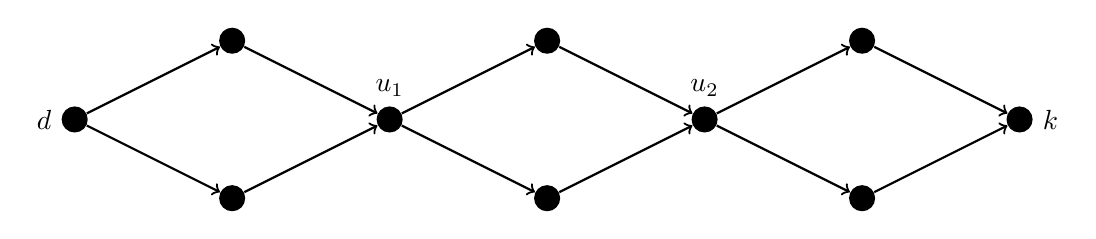
\begin{tikzpicture}
      \coordinate (A) at (0,0);
      \coordinate (B) at (2,1);
      \coordinate (C) at (2,-1);
      \coordinate (D) at (4,0);
      \coordinate (E) at (6,1);
      \coordinate (F) at (6,-1);
      \coordinate (G) at (8,0);
      \coordinate (H) at (10,1);
      \coordinate (I) at (10,-1);
      \coordinate (J) at (12,0);
      
      \node[fill,circle,label=left:{$d$}] (aa) at (A) {};
      \node[fill,circle] (bb) at (B) {};
      \node[fill,circle] (cc) at (C) {};
      \node[fill,circle,label=above:{$u_1$}] (dd) at (D) {};
      \node[fill,circle] (ee) at (E) {};
      \node[fill,circle] (ff) at (F) {};
      \node[fill,circle,label=above:{$u_2$}] (gg) at (G) {};
      \node[fill,circle] (hh) at (H) {};
      \node[fill,circle] (ii) at (I) {};
      \node[fill,circle,label=right:{$k$}] (jj) at (J) {};
      
      \draw[->,thick] (aa) --node {} (bb);
      \draw[->,thick] (aa) --node {} (cc);
      \draw[->,thick] (cc) --node {} (dd);
      \draw[->,thick] (bb) --node {} (dd);
      \draw[->,thick] (dd) --node {} (ee);
      \draw[->,thick] (dd) --node {} (ff);
      \draw[->,thick] (ee) --node {} (gg);
      \draw[->,thick] (ff) --node {} (gg);
      \draw[->,thick] (gg) --node {} (hh);
      \draw[->,thick] (gg) --node {} (ii);
      \draw[->,thick] (hh) --node {} (jj);
      \draw[->,thick] (ii) --node {} (jj);
          
    \end{tikzpicture}
    \caption{first UIP counter example}
    \label{fig:uip}
  \end{figure}
  
  This path in the figure above is a subset of the implication graph. We assume we split this path p into three subset paths. The first path $p_1$ goes from the
  decision node d to the first of the two first UIP's, called $u_1$. The second path $p_2$ goes from $u_1$ to the second first UIP, $u_2$. The third path $p_3$
  goes from $u_2$ to the conflict node k.\\
  The length of the path from the first assumed first UIP $u_1$ to $k$ is $p_2 + p_3$. The length of the path from $u_2$ to k is only $p_3$ and therefore shorter.
  This means there can only be one first UIP, because there cannot be two UIP's with the same shortest length.
  
  }

\item Let $\mathcal{C}$ be a set of clauses and $G$ a conflict graph with
  respect to $\mathcal{C}$. Prove: if a clause $C_l$ is learned following the
  first-UIP scheme, then $C_l$ is a consequence of $\mathcal{C}$.

  \solution{
  
  $C=\{C_1, C_2,... ,C_n\} = \bigwedge_{i=1}^{n} C_i$\\
  \\
  $\pi$ is a variable assignment.\\
  $C \vDash C_l$ iff\\
  $\forall \pi, \pi \vDash C \Rightarrow \pi \vDash C \wedge C_l$\\
  $\forall \pi, \pi \vDash C \Rightarrow \pi \nvDash C \wedge \neg C_l$\\
  \\
  C is satisfiable iff $C \wedge \neg C_l$ is unsatisfiable.\\
  \\
  Proof:\\
  If $C \vdash C_l$ then $C \vDash C_l$ then the deductive system is sound.\\
  \\
  Suppose that C is a countable set of logical formulas then $C \cup \{\neg C_l\}$ is iinconsistent.
  $\Rightarrow C \nvdash C_l$ for some $C_l$.\\
  \\
  By the compactness theorem there $\exists$ a finite subset $C_0 \subseteq \{\neg C_l\}$ is inconsistent (it has no models).\\
  \\
  Then $C_0 \vDash C_l$. ($C_0$ are clauses of the conflict graph)
  
  }
\end{enumerate}


%%%%%%%%%%%%%%%%%%%%%%%%%%%%%%%%%%%%%%%%%%%%%%%%%%%%%%%%%%%%%%%%%%%%%%%%%%%%%%

\newpage
\Aufgabe[Sparse Method \hfill \bf (1.5 points)]
Apply the Sparse Method including preprocessing on the formula $\varphi^E$
below to obtain a propositional formula.
\begin{displaymath}
  (x_1 \neq x_2 \lor x_2=x_3 ) \land \big[ (x_2 \neq x_4 \land x_3=x_4
  \land x_4=x_5)
  \lor (x_6 \neq x_5 \land x_6=x_7 \land x_7=x_3)\big]
\end{displaymath}

  \solution{
We define the above formula as $\varphi^{E}$. We use the Sparse Method to compute  an equisatisfiable formula in propostional logic.
We begin to seperate the formula in equality literals $E_{=}$ and inequality literals $E_{\neq}$. 
\bigskip

$E_{=} = \{x_2 = x_3, x_3 = x_4 , x_4 = x_5 , x_6 = x_7, x_7 =x_3 \}$

\bigskip

$E_{\neq} =\{x_1 \neq x_2, x_2 \neq x_4 , x_6 \neq x_5 \} $

Now we construct the corresponding equality graph $G^{E} (\varphi^{E} )$ :

 \begin{figure}[h]
    \centering
    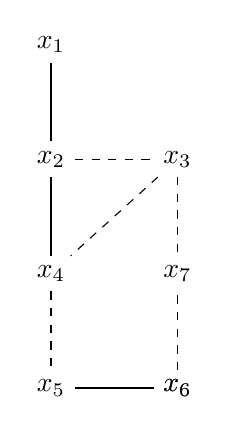
\begin{tikzpicture}
      \node(x1){$x_1$};
      \node[below=of x1](x2){$x_2$};
      \node[right=of x2](x3){$x_3$};
      \node[below=of x2](x4){$x_4$};  
      \node[below=of x4](x5){$x_5$};
      \node[right=of x5](x6){$x_6$};
      \node[below=of x3](x7){$x_7$};
      \node[below=of x7](x6){$x_6$};
      
      
      \draw[] (x1) -- (x2);
      \draw[dashed] (x2) -- (x3);
      \draw[dashed] (x3) -- (x4); 
      \draw[dashed] (x3) -- (x7);
      \draw[] (x2) -- (x4);
      \draw[dashed] (x4) -- (x5);
      \draw[] (x5) -- (x6);
      \draw[dashed] (x6) -- (x7);
 
    \end{tikzpicture}
    \caption{$G^E(\varphi^E)$, dashed lines represent equality, solid lines disequality.}
    \label{fig:sp1}
  \end{figure}

  }

Now we have to search for contradictory cycle. This are cycles which have exactly one dis-equality edge.
Only the Edge $(x_1,x_2)$ are not part of a simple contradictory cycle, therefore we set those edges to $true$ in $\varphi^E$
and obtain $\varphi^E_2$ as:

 \begin{displaymath}
    [ (true \lor  x_2 = x_3 ) \land \big[ (x_2 \neq x_4 \land x_3=x_4
  \land x_4=x_5)
  \lor (x_6 \neq x_5 \land x_6=x_7 \land x_7=x_3)\big]
 \end{displaymath}

  Propositional simplification of $\varphi^E_2$ leads to :
 
 \begin{displaymath}
   \big[ (x_2 \neq x_4 \land x_3=x_4
  \land x_4=x_5)
  \lor (x_6 \neq x_5 \land x_6=x_7 \land x_7=x_3)\big]
 \end{displaymath}

Now we construct the new corresponding equality graph $G^{E} (\varphi^{E_2} )$ :

 \begin{figure}[h]
    \centering
    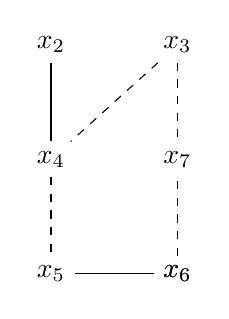
\begin{tikzpicture}
      \node(x2){$x_2$};
      \node[right=of x2](x3){$x_3$};
      \node[below=of x2](x4){$x_4$};  
      \node[below=of x4](x5){$x_5$};
      \node[right=of x5](x6){$x_6$};
      \node[below=of x3](x7){$x_7$};
      \node[below=of x7](x6){$x_6$};
      
      
      \draw[dashed] (x3) -- (x4); 
      \draw[dashed] (x3) -- (x7);
      \draw[] (x2) -- (x4);
      \draw[dashed] (x4) -- (x5);
      \draw[] (x5) -- (x6);
      \draw[dashed] (x6) -- (x7);
 
    \end{tikzpicture}
    \caption{$G^E(\varphi^E_2)$, dashed lines represent equality, solid lines disequality.}
    \label{fig:sp2}
  \end{figure}

\bigskip

Now we have to search again for contradictory cycle.
The Edge $(x_2)$ is not part of a simple contradictory cycle, therefore we set those edges to $true$ in $\varphi^E_2$
and obtain $\varphi^E_3$ as:

\begin{displaymath}
   \big[ (TRUE \land x_3=x_4 \land x_4=x_5)
  \lor (x_6 \neq x_5 \land x_6=x_7 \land x_7=x_3)\big]
 \end{displaymath}
 

  Propositional simplification of $\varphi^E_3$ leads to :
 
 \begin{displaymath}
   \big[ ( x_3=x_4
  \land x_4=x_5)
  \lor (x_6 \neq x_5 \land x_6=x_7 \land x_7=x_3)\big]
 \end{displaymath}


Now are no more nodes not part of a contradictory cycle. So we can build the e propositional skeleton $ e(\varphi^E_3) $ by
  relabeling the equality literals with $e_{i,j}$.


\begin{displaymath}
   \big[ ( e_{3,7} \land e_{4,5} )
  \lor ( \neg e_{6,5} \land e_{6,7} \land e_{7,3})\big]
 \end{displaymath}

The next step is to create a nonpolar version of the graph. To ensure that there are no hidden computational complexity we make the new graph chordal. To do so we have to add some edges at the corresponding nodes like $(x_7,x_5)$ and $(x_3,x_5)$. There are also others possibilities to make the graph chordal. If a graph is chordal then each cycles has the length 3. 

\begin{figure}[h]
    \centering
    \begin{tikzpicture}
      \node(x3){$x_3$};
      \node[left=of x3](x4){$x_4$};  
      \node[below=of x4](x5){$x_5$};
      \node[below=of x3](x7){$x_7$};
      \node[below=of x7](x6){$x_6$};
      
      
      \draw[] (x3) -- (x4); 
      \draw[] (x3) -- (x7);
      \draw[] (x2) -- (x4);
      \draw[] (x4) -- (x5);
      \draw[] (x5) -- (x6);
      \draw[] (x6) -- (x7);
 
    \end{tikzpicture}
    \caption{Non-chordal graph}
    \label{fig:sp3}
  \end{figure}


\begin{figure}[h]
    \centering
    \begin{tikzpicture}
      \node(x3){$x_3$};
      \node[left=of x3](x4){$x_4$};  
      \node[below=of x4](x5){$x_5$};
      \node[below=of x3](x7){$x_7$};
      \node[below=of x7](x6){$x_6$};
      
      
      \draw[] (x3) -- (x4);
      \draw[] (x3) -- (x5);
      \draw[] (x5) -- (x7);
      \draw[] (x3) -- (x7);
      \draw[] (x2) -- (x4);
      \draw[] (x4) -- (x5);
      \draw[] (x5) -- (x6);
      \draw[] (x6) -- (x7);
 
    \end{tikzpicture}
    \caption{Chordal graph}
    \label{fig:sp4}
  \end{figure}

At last we have to derive according transitivity constraints for each triangle to obtain $B_t$.
  
\begin{eqnarray*}
    B_t:= &(e_{3,7} \land e_{3,5} \rightarrow e_{7,5}) \land
   (e_{3,7} \land e_{7,5} \rightarrow e_{3,5}) \land
    (e_{3,5} \land e_{5,7} \rightarrow e_{5,8}) \land & \quad \quad \text{for }\triangle
    (x_3,x_5,x_7)\\
    %
    &(e_{3,4} \land e_{4,5} \rightarrow e_{3,5}) \land
    (e_{4,5} \land e_{3,5} \rightarrow e_{3,4}) \land
    (e_{3,4} \land e_{3,5} \rightarrow e_{4,5}) \land & \quad \quad \text{for
    } \triangle (x_3,x_4,x_5)\\
    %
    &(e_{5,7} \land e_{5,6} \rightarrow e_{6,7}) \land
    (e_{5,7} \land e_{6,7} \rightarrow e_{5,6}) \land
    (e_{5,6} \land e_{6,7} \rightarrow e_{5,7}) &\quad \quad\text{for }  \triangle (x_7,x_5,x_8)
  \end{eqnarray*}

  The sparse Methode generates at the final form  $e(\varphi^E_3) \land B_t$.

  

%%%%%%%%%%%%%%%%%%%%%%%%%%%%%%%%%%%%%%%%%%%%%%%%%%%%%%%%%%%%%%%%%%%%%%%%%%%%%%

\newpage
\Aufgabe[Ackermann's Reduction \hfill \bf (1 point)]
Apply Ackermann's reduction on the following EUF-formula $\varphi$ to obtain
an EU formula:
\begin{displaymath}
  f\left(f\left(g\left(a\right),b\right),a\right) = f(g(a),b) \rightarrow \big[ f(x,y) = g(f(g(a),b)) \land
  g(f(a,y))=d \big]
\end{displaymath}


\solution{
  The first step of the ackermann´s reduction enummerate each variable from outside to inside and from left to right. 
 
 \begin{displaymath}
  f_4\left(f_1\left(g_1\left(a\right),b\right),a\right) = f_1(g_1(a),b) \rightarrow \big[ f_2(x,y) = g_2(f_1(g(a),b)) \land
   g_3(f_3(a,y))=d \big]
 \end{displaymath}

After the enummeration we can define the meanings of the $\cT$:

  \begin{align*}
   \cT (f_1(g_1(a),b)) &= F_1  \\
   \cT (f_2(x,y) &= F_2\\
    \cT (f_3(a,y)) &= F_3 \\
    \cT (f_4(f_1(g_1(a),b),b)) &= F_4 \\
    \cT (g_1(a)) &= G_1\\
    \cT (g_2(f_1(g_1(a),b)) &= G_2 \\
    \cT (g_3(f_3(a,y)) &= G_3  \\ 
  \end{align*}

After we defined $\cT$ we can write the $flat^E$.

$ flat^E:= F_3 = F_1 \rightarrow  (F_2 = G_2) \land G_3 = d $. 
In the next step we construct the functional consistency constraints $FC^E$ as follows:
 
 \begin{align*}
  FC^E := \\
    ((a = F_1) \rightarrow & G_1 = G_2) \land \\
     ((a = F_2) \rightarrow & G_1 = G_3) \land \\
      ((F_1 = F_2) \rightarrow & G_2 = G_3) \land \\
      ((G_1 = x \land b=y) \rightarrow & F_1 = F_2) \land \\
      ((G_1 = a \land b=y ) \rightarrow & F_1 = F_3) \land \\
      ((G_1 = F_1 \land b=a) \rightarrow & F_1 = F_2) \land \\
      ((x = a \land y=y) \rightarrow & F_2 = F_3) \land \\
      ((x= F_1 \land y=a) \rightarrow & F_2 = F_4) \land \\
      ((a = F_1 \land y=a) \rightarrow & F_3 = F_4))
 \end{align*}


Finally, the we generate the equality formula : $\varphi^E := FC^E \rightarrow flat^E$

}


\end{document}
